%%%%%%%%%%%%%%%%%%%%%%%%%%%%%%%%%%%%%%%%%
% Beamer Presentation
% LaTeX Template
% Version 1.0 (10/11/12)
%
% This template has been downloaded from:
% http://www.LaTeXTemplates.com
%
% License:
% CC BY-NC-SA 3.0 (http://creativecommons.org/licenses/by-nc-sa/3.0/)
%
%%%%%%%%%%%%%%%%%%%%%%%%%%%%%%%%%%%%%%%%%

%----------------------------------------------------------------------------------------
%	PACKAGES AND THEMES
%----------------------------------------------------------------------------------------

\documentclass{beamer}

\mode<presentation> {

% The Beamer class comes with a number of default slide themes
% which change the colors and layouts of slides. Below this is a list
% of all the themes, uncomment each in turn to see what they look like.

%\usetheme{default}
%\usetheme{AnnArbor}
%\usetheme{Antibes}
%\usetheme{Bergen}
%\usetheme{Berkeley}
%\usetheme{Berlin}
%\usetheme{Boadilla}
\usetheme{CambridgeUS}
%\usetheme{Copenhagen}
%\usetheme{Darmstadt}
%\usetheme{Dresden}
%\usetheme{Frankfurt}
%\usetheme{Goettingen}
%\usetheme{Hannover}
%\usetheme{Ilmenau}
%\usetheme{JuanLesPins}
%\usetheme{Luebeck}
%\usetheme{Madrid}
%\usetheme{Malmoe}
%\usetheme{Marburg}
%\usetheme{Montpellier}
%\usetheme{PaloAlto}
%\usetheme{Pittsburgh}
%\usetheme{Rochester}
%\usetheme{Singapore}
%\usetheme{Szeged}
%\usetheme{Warsaw}

% As well as themes, the Beamer class has a number of color themes
% for any slide theme. Uncomment each of these in turn to see how it
% changes the colors of your current slide theme.

%\usecolortheme{albatross}
%\usecolortheme{beaver}
%\usecolortheme{beetle}
%\usecolortheme{crane}
\usecolortheme{dolphin}
%\usecolortheme{dove}
%\usecolortheme{fly}
%\usecolortheme{lily}
%\usecolortheme{orchid}
%\usecolortheme{rose}
%\usecolortheme{seagull}
%\usecolortheme{seahorse}
%\usecolortheme{whale}
%\usecolortheme{wolverine}

%\setbeamertemplate{footline} % To remove the footer line in all slides uncomment this line
%\setbeamertemplate{footline}[page number] % To replace the footer line in all slides with a simple slide count uncomment this line

\setbeamertemplate{navigation symbols}{} % To remove the navigation symbols from the bottom of all slides uncomment this line
}

\usepackage{graphicx} % Allows including images
\usepackage{booktabs} % Allows the use of \toprule, \midrule and \bottomrule in tables
\usepackage{listings} % For code


\definecolor{verylightgray}{rgb}{.97,.97,.97}

\lstdefinelanguage{Solidity}{
	keywords=[1]{anonymous, assembly, assert, balance, break, call, callcode, case, catch, class, constant, continue, constructor, contract, debugger, default, delegatecall, delete, do, else, emit, event, experimental, export, external, false, finally, for, function, gas, if, implements, import, in, indexed, instanceof, interface, internal, is, length, library, log0, log1, log2, log3, log4, memory, modifier, new, payable, pragma, private, protected, public, pure, push, require, return, returns, revert, selfdestruct, send, solidity, storage, struct, suicide, super, switch, then, this, throw, transfer, true, try, typeof, using, value, view, while, with, addmod, ecrecover, keccak256, mulmod, ripemd160, sha256, sha3}, % generic keywords including crypto operations
	keywordstyle=[1]\color{blue}\bfseries,
	keywords=[2]{address, bool, byte, bytes, bytes1, bytes2, bytes3, bytes4, bytes5, bytes6, bytes7, bytes8, bytes9, bytes10, bytes11, bytes12, bytes13, bytes14, bytes15, bytes16, bytes17, bytes18, bytes19, bytes20, bytes21, bytes22, bytes23, bytes24, bytes25, bytes26, bytes27, bytes28, bytes29, bytes30, bytes31, bytes32, enum, int, int8, int16, int24, int32, int40, int48, int56, int64, int72, int80, int88, int96, int104, int112, int120, int128, int136, int144, int152, int160, int168, int176, int184, int192, int200, int208, int216, int224, int232, int240, int248, int256, string, uint, uint8, uint16, uint24, uint32, uint40, uint48, uint56, uint64, uint72, uint80, uint88, uint96, uint104, uint112, uint120, uint128, uint136, uint144, uint152, uint160, uint168, uint176, uint184, uint192, uint200, uint208, uint216, uint224, uint232, uint240, uint248, uint256, var, void, ether, finney, szabo, wei, days, hours, minutes, seconds, weeks, years},	% types; money and time units
	keywordstyle=[2]\color{teal}\bfseries,
	keywords=[3]{block, blockhash, coinbase, difficulty, gaslimit, number, timestamp, msg, data, gas, sender, sig, value, now, tx, gasprice, origin, mapping},	% environment variables
	keywordstyle=[3]\color{violet}\bfseries,
	identifierstyle=\color{black},
	sensitive=true,
	comment=[l]{//},
	morecomment=[s]{/*}{*/},
	commentstyle=\color{gray}\ttfamily,
	stringstyle=\color{red}\ttfamily,
	morestring=[b]',
	morestring=[b]"
}

\lstset{
	language=Solidity,
    extendedchars=true,
    backgroundcolor=\color{verylightgray},
	basicstyle=\footnotesize\ttfamily,
	showstringspaces=false,
	showspaces=false,
	tabsize=3,
	breaklines=true,
	showtabs=false,
	captionpos=b
}

%----------------------------------------------------------------------------------------
%	TITLE PAGE
%----------------------------------------------------------------------------------------

\title[]{La gestione di ruoli e permessi sulla blockchain Ethereum}

\date{23 settembre 2019}

\titlegraphic{
\includegraphics[width=0.4\linewidth]{img/logo_unitn_black_center.eps}}

\author{Matteo Golinelli}

\def\coauthors{Prof. Alberto Montresor}

\institute[UniTN]

\begin{document}

%\begin{frame}
%\titlepage % Print the title page as the first slide
%\end{frame}


%------------------------------------------------

\begin{frame}

\begin{center}

\begin{figure}

\includegraphics[width=0.5\linewidth]{img/logo_unitn_black_center.eps}
\end{figure}

\footnotesize Corso di Laurea in Informatica

\begin{center}
\usebeamerfont*{frametitle}
\usebeamercolor[fg]{frametitle}
\begin{block}{}
\centering
La gestione di ruoli e permessi sulla \\ blockchain Ethereum
\end{block}
\end{center}

\begin{tabular*}{\textwidth}{ c @{\extracolsep{\fill}} c }
\small Supervisore & \small Laureando\\
Prof. Alberto Montresor& Matteo Golinelli\\
\end{tabular*}

\vspace{.5 cm}

\scriptsize{Anno accademico 2018/2019}

\end{center}


\end{frame}


%----------------------------------------------------------------------------------------
%	PRESENTATION SLIDES
%----------------------------------------------------------------------------------------

\begin{frame}
\frametitle{Digicando}

Fornisce servizi di:

\begin{itemize}
    \item Anticontraffazione, certificazione e tracciabilità di prodotti
    \item Analisi statistica sugli acquirenti dei prodotti
    \item Recensioni affidabili e certificate
\end{itemize}

\end{frame}

%------------------------------------------------

\begin{frame}
\frametitle{Architettura}

\begin{block}{Attuale}
L'architettura dell'implementazione attuale del servizio di Digicando è \emph{client-server}
\end{block}

\begin{block}{Futura}
L’obiettivo di Digicando è spostare il servizio di anticontraffazione sulla \emph{Blockchain Ethereum}
\end{block}

\end{frame}

%------------------------------------------------

\begin{frame}
\frametitle{Motivazioni}
L'utilizzo della tecnologia blockchain fornisce un'infrastruttura in grado di registrare e certificare i trasferimenti di proprietà di un prodotto in maniera:

\begin{itemize}
    \item Sicura
    \item Immodificabile
    \item Trasparente
    \item Aperta al controllo di chiunque
\end{itemize}

\end{frame}

%------------------------------------------------

\begin{frame}
\frametitle{Svantaggi}
L'utilizzo della blockchain introduce una serie di problematiche:

\begin{itemize}
    \item Mancanza del concetto di segretezza
    \item Scalabilità della blockchain stessa
    \item Possibile introduzione di leggi che limitino le possibilità di utilizzo delle criptovalute
\end{itemize}

\end{frame}

%------------------------------------------------

\begin{frame}
\frametitle{Blockchain}

\begin{itemize}
    \item La Blockchain è una struttura dati \emph{distribuita}
    \item Ha come obiettivo il mantenimento di un registro immodificabile e crescente
    \item Il registro è composto da blocchi, connessi utilizzando la crittografia
\end{itemize}

\end{frame}

%------------------------------------------------

\begin{frame}
\frametitle{Blockchain}

Ogni blocco contiene:
\begin{itemize}
    \item Un hash crittografico del blocco precedente
    \item Un timestamp
    \item Dati riguardanti delle transazioni
\end{itemize}

\begin{figure}
\includegraphics[width=0.9\linewidth]{img/blockchain}
\end{figure}

\end{frame}

%------------------------------------------------

\begin{frame}
\frametitle{Blockchain}

La blockchain è:

\begin{block}{Distribuita}
    Si dice distribuita in quanto ogni partecipante alla rete ne condivide una copia identica
\end{block}

\begin{block}{Immodificabile}
    Una blockchain è immodificabile per definizione, in quanto ogni
    modifica invaliderebbe crittograficamente l’intera struttura
\end{block}

\end{frame}

%------------------------------------------------

\begin{frame}
\frametitle{Ethereum}

\begin{itemize}
    \item Ethereum è una blockchain open-source con criptovaluta nativa chiamata \emph{Ether}
    \item L'Ether è una moneta digitale non è controllata da alcun governo o azienda
    \item Ethereum è programmabile:
    \begin{itemize}
        \item E' possibile sviluppare ed eseguire applicazioni decentralizzate (\emph{DApp})
        \item Beneficiano della criptovaluta e della tecnologia blockchain
    \end{itemize}
\end{itemize}

\end{frame}

%------------------------------------------------

\begin{frame}
\frametitle{Problema}

\begin{itemize}
    \item Durante la fase di sviluppo dell’applicazione si è data priorità allo sviluppo del core dell’applicazione
    \item Alcune caratteristiche e funzioni sono state tralasciate per il futuro
    \item La principale limitazione è l'impossibilità di gestire i contratti da più indirizzi
    \begin{itemize}
        \item Costringe a mantenere una chiave privata condivisa
        \item Limita la flessibilità del sistema nell'aggiunta e rimozione degli utenti autorizzati
    \end{itemize}
\end{itemize}

\end{frame}

%------------------------------------------------

\begin{frame}
\frametitle{Problema}

\begin{itemize}
    \item Inizialmente la gestione dei ruoli è stata realizzata mediante un sistema di \emph{whitelisting} all'interno dei contratti stessi
    \item Irrigidisce l'architettura nel momento di eventuali aggiornamenti dei contratti
    \item Aumenta la complessità dei contratti interessati, costretti a svolgere compiti non correlati al loro scopo
\end{itemize}

\end{frame}

%------------------------------------------------

\begin{frame}
\frametitle{Requisiti}
I requisiti del sistema più importanti individuati insieme all'azienda sono:

\begin{itemize}
    \item Il sistema deve lavorare interamente su blockchain
    \item Il sistema deve essere dinamico sulla creazione di nuovi ruoli
    \item I ruoli devono poter essere gestiti in maniera gerarchica
\end{itemize}

\end{frame}

%------------------------------------------------

\begin{frame}
\frametitle{Soluzione}

La soluzione individuata prevede:
\begin{itemize}
    \item Due contratti esterni, in sostituzione del sistema di whitelisting degli indirizzi
    \item Un approccio basato su claim
    \begin{itemize}
        \item Gli utenti possono attribuire claim ad altri utenti
        \item Le claim conferiscono particolari privilegi
    \end{itemize}
\end{itemize}

\end{frame}

%------------------------------------------------

\begin{frame}
\frametitle{Tecnologie utilizzate}

Le tecnologie utilizzate per lo sviluppo del sistema sono open-source e sono:

\begin{itemize}
    \item \emph{Solidity}: linguaggio di programmazione per la blockchain Ethereum
    \item \emph{Truffle}: ambiente di sviluppo, framework per il testing, insieme di risorse
    \item \emph{Ganache}: strumento per la creazione di blockchain personali per il testing
\end{itemize}

\end{frame}

%------------------------------------------------

\begin{frame}
\frametitle{Contratti}

\begin{block}{ClaimsRegister}
    \begin{itemize}
        \item Implementa un registro che memorizza i ruoli emessi, cioè le \emph{claim}
        \item Implementa una funzione per il controllo di validità delle singole claim ed una per la loro rimozione
    \end{itemize}
\end{block}

\end{frame}

%------------------------------------------------

\begin{frame}
\frametitle{Contratti}

\begin{block}{ClaimsManagement}
    Permette di gestire delle strutture organizzative gerarchiche e complesse
\end{block}

\begin{figure}[]
    \begin{minipage}[c]{0.5\textwidth}
        \centering
        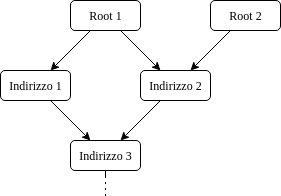
\includegraphics[scale=2]{img/gerarchia.png}
    \end{minipage}\hfill
    \begin{minipage}[c]{0.5\textwidth}
        \caption{Un esempio di gerarchia complessa} \label{fig:03-03}
    \end{minipage}
\end{figure}

\end{frame}

%------------------------------------------------

\begin{frame}[fragile]
\frametitle{Registro}

Il registro è un \texttt{mapping}, cioè una tabella hash nel linguaggio Solidity.

Memorizza un valore associato a tre chiavi:

\begin{itemize}
    \item \emph{Emitter}: l'indirizzo che emette il ruolo
    \item \emph{Receiver}: l'indirizzo che riceve il ruolo
    \item \emph{Claim}: la chiave di un ruolo
\end{itemize}

\begin{lstlisting}[language=Solidity]
    // emitter => receiver => claim => value
    mapping(address => mapping(address => mapping(bytes32 => bytes32))) public registry;
\end{lstlisting}

\end{frame}

%------------------------------------------------

\begin{frame}[fragile]
\frametitle{Integrazione}

Fasi del processo di integrazione:

\begin{itemize}
    \item Studio dell'implementazione attuale
    \item Individuazione dei contratti che fanno uso del sistema di whitelisting
    \item Sostituzione del vecchio sistema con il nuovo
    \item Testing approfondito del sistema integrato
\end{itemize}

\end{frame}

%------------------------------------------------

\begin{frame}
\frametitle{Conclusioni}

\begin{itemize}
    \item Il sistema sviluppato, composto dai due contratti, ha risolto il problema
    \item Il sistema di Digicando così integrato risulta più flessibile, funzionale e performante
\end{itemize}

\end{frame}

%------------------------------------------------

%----------------------------------------------------------------------------------------

\end{document} 